\graphicspath{ {./Images/} }

\section{Prerequisites}
This section is dedicated to refreshing your understanding of key concepts that are not technically part of control theory, but are nonetheless necessary in order to understand it. In addition, this section includes some basic instructions of how DSLs work in practice.

These subjects are only touched upon on a very basic level, thus if you are already feeling confident about them, this section can be safely skipped.

\subsection{Complex numbers}
\iffalse
Här är målet främst att introducera dsl som koncept och även introducera hur vi behandlar komplexa tal eftersom detta kommer återkomma mycket i texten. Vi gör detta genom att snabbt repetera komplexa tal. Vi antar dock att läsaren egentligen är bekväm med komplexa tal och att detta istället är en mjukstart för dsl, haskell och våra egna betäckningar.\\
\fi

In short, the complex numbers are an extension of the real numbers in the same way that the real numbers are an extension of the rational numbers. With the reals, we saw the addition of a number of constants(e, $\pi$, etc.).
This time around, we add imaginary numbers.

First, some technicalities. The complex numbers are built on the real numbers, but the real numbers are unfortunately not very easily implementable in computers. In reality we have to approximate. In order to avoid this problem, we're going to introduce a type synonym: 

\begin{minted}{haskell}
type R = Double 
\end{minted}
%\todo{Real är upptaget i haskell}

Now, whenever we want something to be a real number, we can use the type \cmd{R}. Type synonyms are just that --- synonyms --- so whenever you see \cmd{R} throughout the text you could exchange it with \cmd{Double} and get the exact same result. We hope you see the reason in using \cmd{R}, however. 
%Note that the doubles are inherently inaccurate; they cannot provide more than an approximation of most non-integers(I.E. 2/3, e, $\pi$, etc.). Since we are more concerned with understanding the process than getting a strictly accurate answer, however, this simplification is quite alright.

\subsubsection{The Imaginary Number Concept}
So what are imaginary numbers? 
In short, imaginary numbers are a way to solve some equations that are otherwise impossible to solve. For example, if we wanted to find a root to -1 we'd need to use imaginary numbers. 

%In short, imaginary numbers are the pet project of some scientist who really really wanted a root to -1. This then turned into an entire field of study.

Let's start with the definition:
\begin{align*}
    i = \sqrt{-1},
\end{align*}
or put otherwise, 
\begin{align*}
    i^2 = -1.
\end{align*}

What we've got so far is just one number. So what? Well, let's look at what we can do with them. 

Imaginary numbers have a tendency to show up alongside real numbers. As such, mathematicians have standardized complex numbers as being read ``a + bi.'' Some examples of complex numbers written this way are $2+3i$, $\pi + ei$ and $1+0i$. 
We'll get back to that soon, but first we want to introduce our own representation. 

%Rather than bother with this expression, however, we are going to ignore it and instead create our own using the power of programming:
\begin{minted}{haskell}
data Complex = Complex (R, R)
    deriving (Show)
\end{minted}

This is the first step to creating a domain-specific language: establishing how our `words' (or in this case numbers) are written. We create a data type called \cmd{complex}, which holds a pair of values. 

Now you might ask yourself: why did we choose to put our doubles in parenthesis? The answer lies in the complex plane and how complex numbers can be seen as coordinates in a diagram. For example, see the following figure:
%To help explain how we're actually going to use complex numbers going forwards (for the most part, anyway). Behold, the Argand diagram!

\begin{figure}[h!]
    \centering
    \includegraphics[scale= 0.4]{Argand.png}
    \caption{}
    \label{argand}
\end{figure}


In the picture you see a complex plane with the complex number $(7,6i)$ marked. Note the similarity to coordinate planes. TODO: write a little more about how real works like x and im as y. 
%You may notice a similarity to coordinate planes. This is because they are essentially the same. 
%This is because they are essentially one and the same.
%Also note how we wrote our datatype to imitate how coordinates are usually written. We are very smart.

\subsubsection{Basic Operators}

For our first operators, let's just create a pair of functions that extract the real and imaginary parts of the Complex number. As can be seen in the picture above, the real numbers exist along the x-axis, and the imaginary ones exist along the y-axis. As such:
\begin{minted}{haskell}
whatsReal :: Complex -> R
whatsReal (Complex (x,y)) = x

\end{minted}
%whatsImaginary :: Complex -> Real
% whatsImaginary (Complex (x,y)) = y

\begin{exercise}
Implement the other function, \cmd{whatsImaginary :: Complex -> Real}. 
\end{exercise}

Well, that was easy enough. Note that had we chosen a different representation of complex numbers, say the polar one, these would be a little harder. 

%Now, as practiced Haskellians, you might wonder what we can do with these complex numbers. So far, our datatype does not really behave like numbers -- we can't add them to each other, for example. Thus a lot of what we want to do can be seen as implementing a Num instance. 
First, let's define the most fundamental of all math operators: addition. Please look at the picture below.

\begin{figure}[h!]
    \centering
    \includegraphics[scale= 0.4]{Addition.png}
    \caption{Addition of two complex numbers $z$ and $w$, and the resulting number $v$.}
    \label{addition}
\end{figure}

In the picture we see the complex numbers $z, w$ and $v$. We want adding them to behave like adding two points in a graph: the result of going from the origin to one of the points and then following the other from there. For example, in \ref{addition}, we see that $v = z + w$, because we can go from the origin to $(9,2i)$ and then follow $(3,6i)$ from there. 

When working in rectangular form we can implement addition similar to how it works with Cartesian coordinates: add reals to reals and imaginaries to imaginaries. Since we represent our complex numbers as a pair, we only have to add the components of the pair to each other: 
%This is the first instance of our coordinate-esque DSL making calculation simple. We can clearly see that to add two Complex numbers together, we add reals to reals, and imaginaries to imaginaries. To wit:
\begin{minted}{haskell}
add :: Complex -> Complex -> Complex
add (Complex (r1,i1)) (Complex (r2,i2)) = (Complex (r1+r2,i1+i2))
\end{minted}

Note that addition was easy to implement because of our choice of coordinates.  

Next, let's add subtraction. This works according to the same principle as addition, where real affects real and imaginary affects imaginary.   
\begin{minted}{haskell}
sub :: Complex -> Complex -> Complex
sub (Complex (r1,i1)) (Complex (r2,i2)) = Complex (r1-r2,i1-i2)
\end{minted}

\subsubsection{Imaginary Geometry}

Now, let's move on to the main reason why we chose to mimic coordinates when defining our datatype. No, it wasn't to simplify addition and subtraction. That was just a bonus.

The real reason is that it allows us to use complex numbers to express geometry. To do this, we'll need two core functions. First off, the absolute value.

Note that, since complex numbers exist on a plane rather than a line, we can't just turn them positive and call it a day. Instead, we'll have to call upon our good old friend Pythagoras:

\begin{figure}[h!]
    \centering
    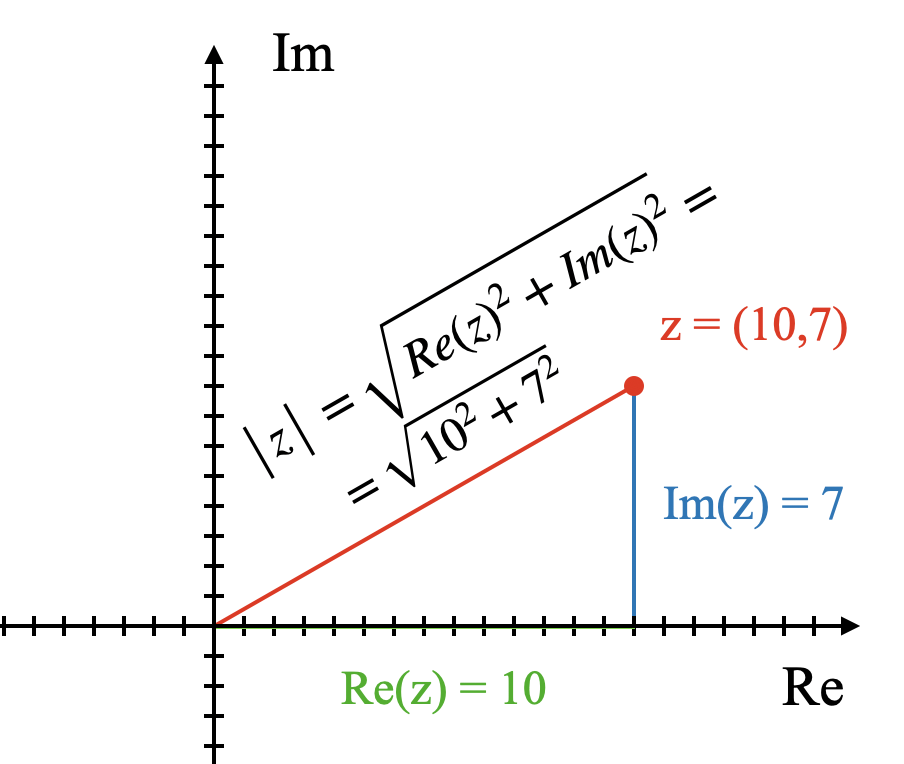
\includegraphics[scale= 0.4]{abs.png}
    \caption{}
    \label{abs}
\end{figure}

\begin{minted}{haskell}
absolute :: Complex -> R
absolute (Complex (real,imaginary)) = sqrt (real^2 + imaginary^2)
\end{minted}
Since squaring always result in positive values, there's no need to worry about whether the values started out positive or negative.\\
Let's move on to arguments, a.k.a. angles.

Pythagoras' theorem is not the only geometric rule that can be combined with complex diagrams/coordinates. In fact, all of them can. Let's do some tangents. Except when working with complex numbers, the resulting value is called an argument rather than an angle.

Unlike regular angles, however, the standard way to express a complex argument, also known as the ''Principal Argument'' does not include a complete 360degree circle from positive real to positive real. Instead, the principal argument uses two scales from the positive reals to the negative reals. One covers positive imaginary values and gives arguments ranging from 0 to $\pi$. The other covers negative imaginaries and gives arguments ranging from 0 to $-\pi$. See picture below for clarity.

\begin{figure}[h!]
    \centering
    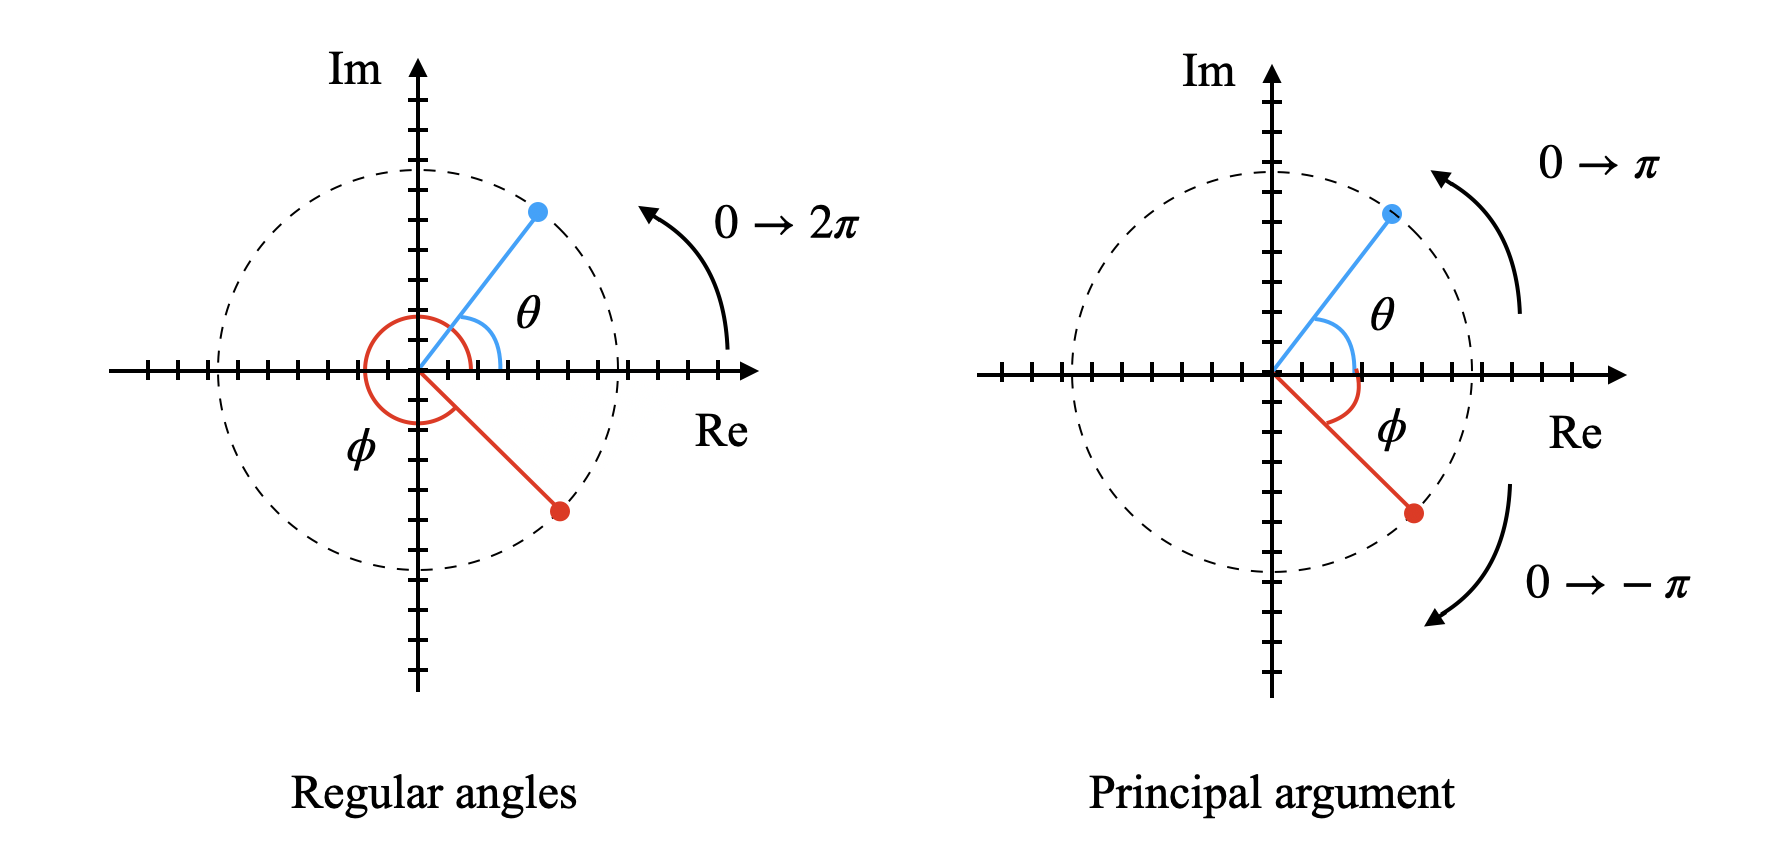
\includegraphics[scale= 0.45]{arg.png}
    \caption{}
    \label{arg}
\end{figure}

The good news is that the arcus tangent(arctan) operator supports this split natively. The bad news is that the arcusTangent operator input only describes the depression of the line; the koefficient.

As illustrated just below, what we'll have to do is program the operator to determine which quadrant the complex number is in, and ''spin'' the resulting argument accordingly.

\begin{figure}[h!]
    \centering
    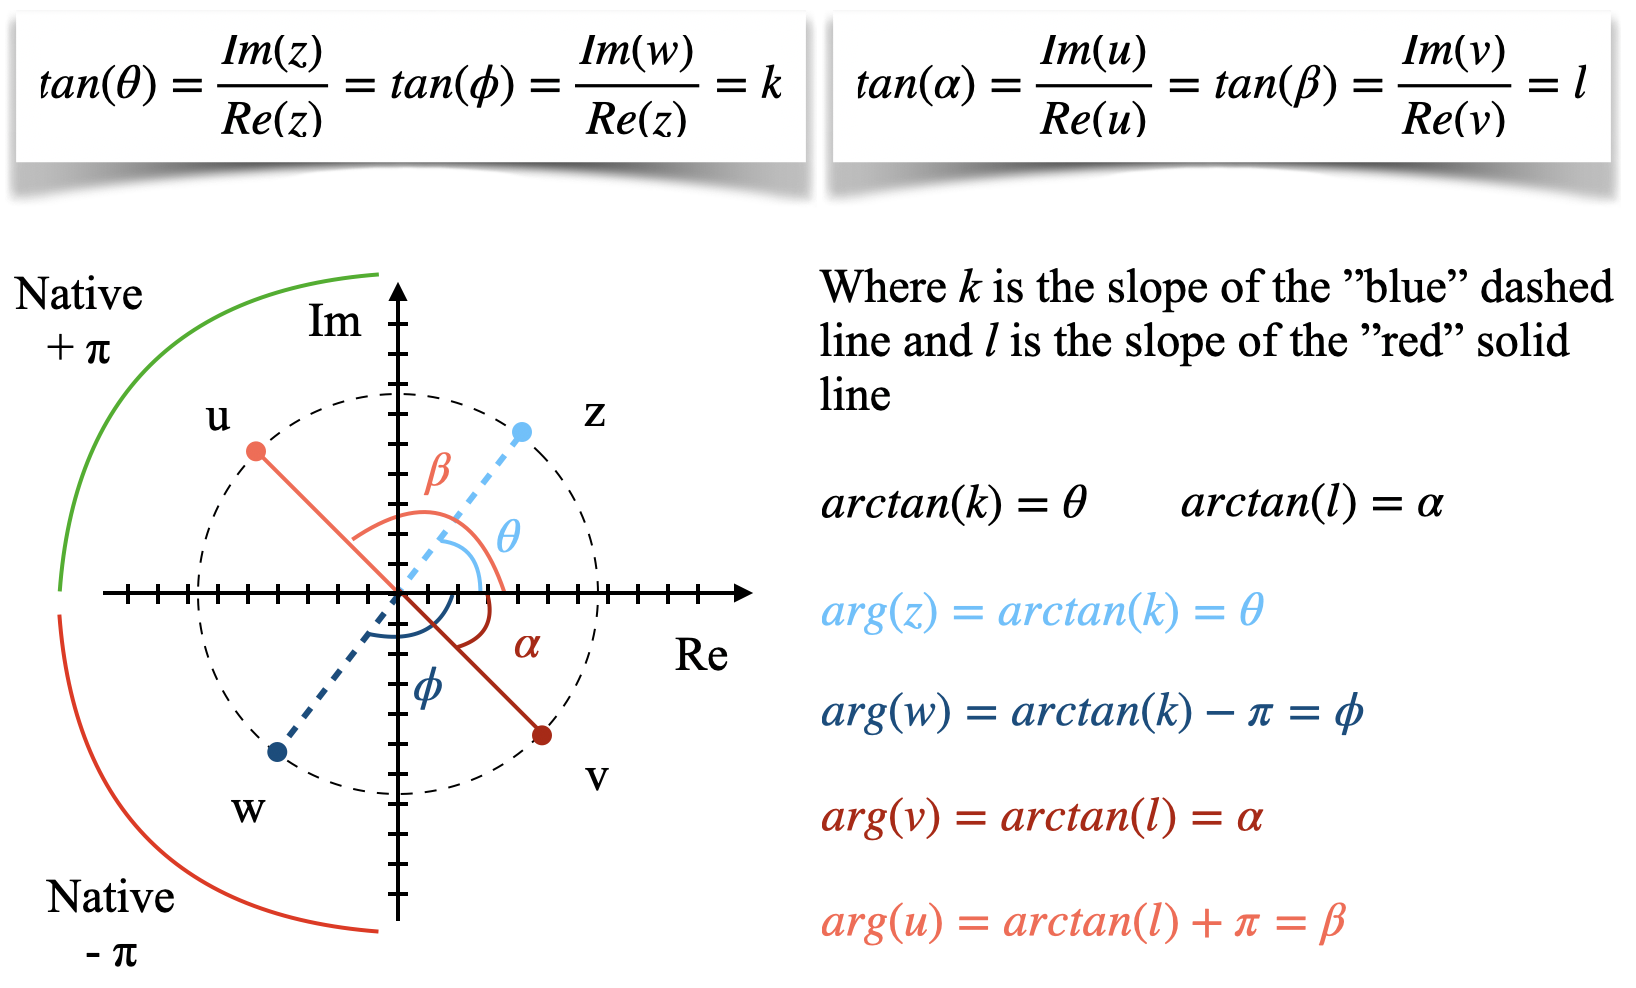
\includegraphics[scale= 0.5]{tan.png}
    \caption{}
    \label{tan}
\end{figure}

\begin{minted}{haskell}
argument :: Complex -> Double
argument (Complex (real,imaginary))
  | real < 0 && imaginary > 0  = (atan (imaginary/real)) + pi
  | real < 0                   = (atan (imaginary/real)) - pi
  | otherwise                  = atan (imaginary/real)
\end{minted}

Please note that our function is currently undefined whenever the real component is zero, due to division by zero. We could solve this with a further three lines describing specific cases for +90$^{\circ}$, -90$^{\circ}$, and true zero. In this case we chose not to in order to keep our code as clean as possible. Alternatively, we could've just used Haskells builtin version of the operator above, known as \cmd{atan2}. If we were lazy, that is. Which we are not.
\vspace{5mm}

The Absolute Value and the Principal Argument, with their powers combined, form an alternate way to express the ''position'' of a Complex number; by expressing the direction and distance from the origin. The later sections will have a field day exploring the possibilities of this, but for now let's move on.

\subsubsection{Advanced Operators}

There is one final function that awaits us; one final operator:\\ multiplication!\\
..\\
Ok, might not sound like much, but there's a reason why we're tackling it last.\\
Can you tell us how to multiply two Complex numbers, based on what we've been talking about so far?\\
..\\
The simple truth of the matter is, we can't. Each Domain-specific Language is, as the name suggests, only meant to express one domain. Our chosen domain was geometry, and we chose to express our Complex numbers as coordinates to aid with that.

That does not mean we can't build a function to multiply two Complex numbers, but it does mean we'll have to move outside the bounds of our DSL to accomplish it.

To wit; in regular math, complex numbers are normally written on the form ''a + bi'', I.E. reals + imaginaries. With that language in mind, basic algebra become a lot more intuitive. 'multiply Complex (r1,i1) Complex (r2,i2)' in our DSL becomes (r1 + i1)(r2 + i2). This can be solved the same way we solve any multiplication of additions; by multiplying each combination and adding the results:

\begin{figure}[h!]
    \centering
    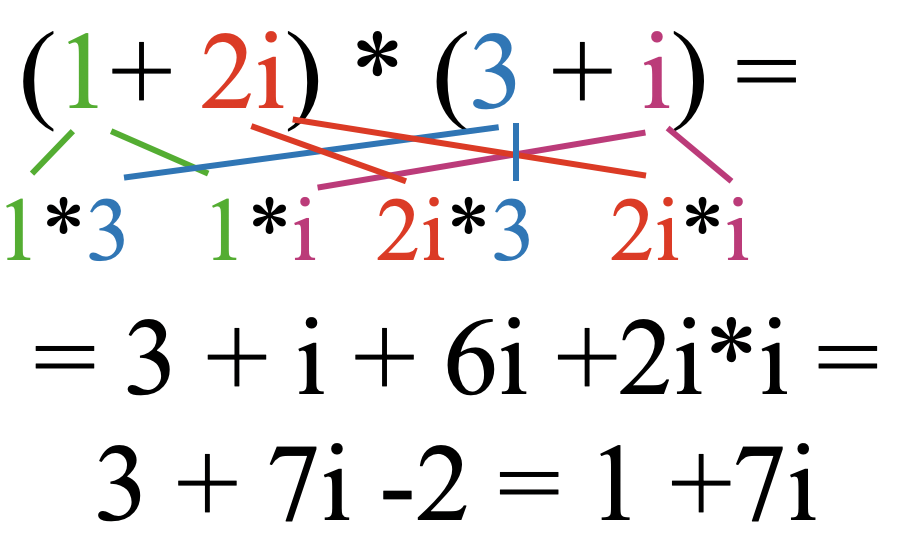
\includegraphics[scale= 0.3]{mult.png}
    \caption{}
    \label{mult}
\end{figure}

As such, by cleverly switching languages, we can find solutions to problems that our current DSL struggles with.

We can now define an operator in our own DSL using the information provided by traditional algebra to reach a correct answer. There is still one annoying complication remaining, however; we've got one term containing $i^2$. How will we make that work with how we've defined our datatype? We never added a way to write powers!

Ach, if only there was a convenient comment regarding the definition of i that we brought up at the beginning of the section and fully expect you to have forgotten about.

\begin{figure}[h!]
    \centering
    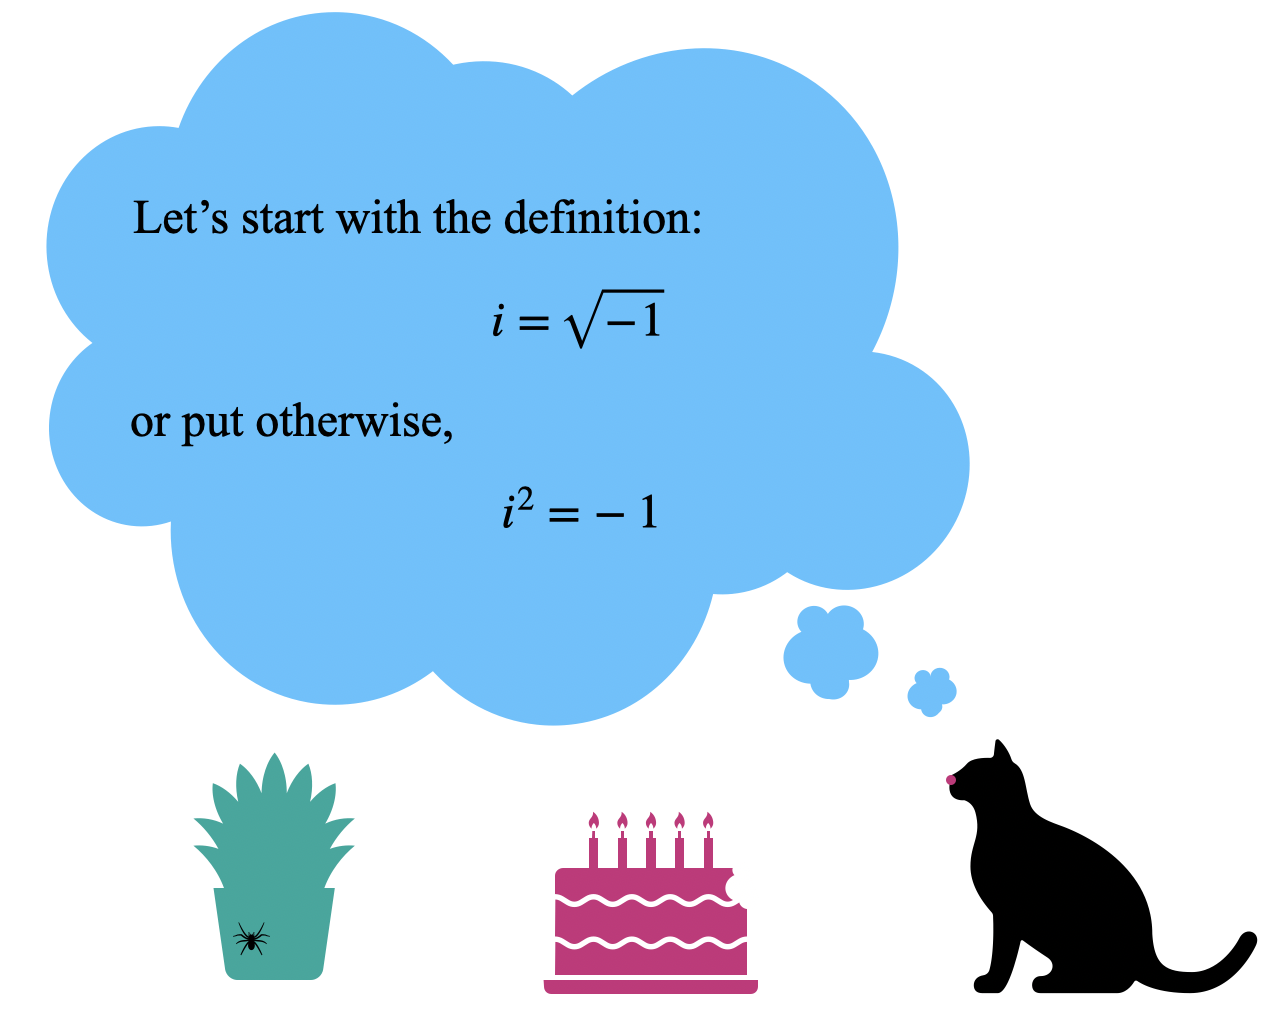
\includegraphics[scale= 0.4]{catretrospective.png}
    \caption{}
    \label{catretro}
\end{figure}

Oh wait, there is just such a thing! $i^2$ is the same as -1! We can now complete our final function and also operator.

\begin{minted}{haskell}
multiply :: Complex -> Complex -> Complex
multiply (Complex (r1,i1)) (Complex (r2,i2))
  = Complex (r1*r2 - i1*i2, r1*i2 + r2*i1)
\end{minted}
This code may look a bit overwhelming, but it's quite simple, really. We're just inserting the rule from basic algebra above, except with the final $i^2$ expression replaced with a negation, in accordance with the definition of i.

\vspace{1cm}

TODO: Mention that this was a fairly shallow dsl. Write a little about how using polar coordinates would make some stuff easier and some harder, show how by giving alternative definitions of (some of?) the functions. Maybe implement it as a Num instance? 

As noted at the very top, complex numbers are an entire field of study. If we were to cover all there is to know about them, this section would take up a small library worth of text and require an actual budget to write. The above should be just enough to give a basic understanding of the concept, along with all operators used in the sections below. Just remember that the coordinate comparison, while undeniably useful, does not apply to every possible operation and you'll do fine.

\subfile{Integrals}


\iffalse %% OLD %%
\begin{code}
data Complex = Complex (Double, Double)
  deriving (Show)
  
test1 = Complex (1,1)
test2 = Complex (3,4)

whatsReal :: Complex -> Double
whatsReal (Complex (x, y)) = x

whatsImaginary :: Complex -> Double
whatsImaginary (Complex (x, y)) = y

add :: Complex -> Complex -> Complex
add (Complex (r1,i1)) (Complex (r2,i2)) = (Complex (r1+r2,i1+i2))

sub :: Complex -> Complex -> Complex
sub (Complex (r1,i1)) (Complex (r2,i2)) = Complex (r1-r2,i1-i2)

absolute :: Complex -> Double
absolute (Complex (real,imaginary)) = sqrt (real^2 + imaginary^2)

argument :: Complex -> Double
argument (Complex (real,imaginary))
  | real < 0 && imaginary > 0  = (atan (imaginary/real)) + pi
  | real < 0                   = (atan (imaginary/real)) - pi
  | otherwise                  = atan (imaginary/real)
  
multiply :: Complex -> Complex -> Complex
multiply (Complex (r1,i1)) (Complex (r2,i2))
  = Complex (r1*r2 - i1*i2, r1*i2 + r2*i1)

\end{code}
\fi